\documentclass{article}

\usepackage[paperwidth=450pt,paperheight=230pt,margin=0pt]{geometry}
\usepackage[T1]{fontenc}
\usepackage[utf8]{inputenc}
\usepackage{lmodern}
\usepackage{xcolor}
\usepackage{tikz}

\definecolor{cutlass}{gray}{0}
\definecolor{ltline}{gray}{0}
\definecolor{gridline}{gray}{0.85}
\definecolor{axisline}{gray}{0.45}

\pagestyle{empty}
\setlength{\parindent}{0pt}

\begin{document}
\noindent
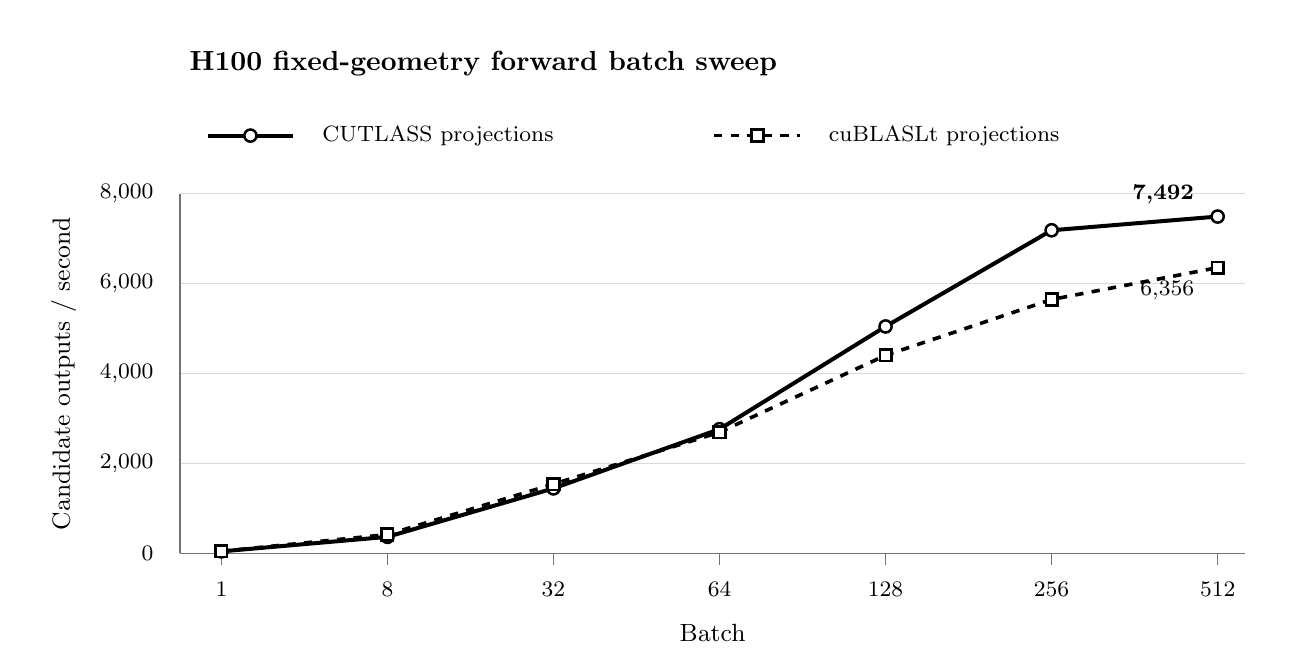
\begin{tikzpicture}[x=1pt,y=1pt]
  \useasboundingbox (0,0) rectangle (450,220);
  \fill[white] (0,0) rectangle (450,220);

  \node[anchor=west,font=\bfseries\fontsize{10}{12}\selectfont]
    at (55,207) {H100 fixed-geometry forward batch sweep};

  \foreach \y/\label in {30/{0},62.5/{2,000},95/{4,000},127.5/{6,000},160/{8,000}} {
    \draw[gridline,line width=0.45pt] (55,\y) -- (440,\y);
    \node[anchor=east,font=\fontsize{8}{9}\selectfont] at (49,\y) {\label};
  }

  \draw[axisline,line width=0.7pt] (55,30) -- (55,160);
  \draw[axisline,line width=0.7pt] (55,30) -- (440,30);

  \foreach \x/\label in {70/{1},130/{8},190/{32},250/{64},310/{128},370/{256},430/{512}} {
    \draw[axisline,line width=0.55pt] (\x,30) -- (\x,26);
    \node[anchor=north,font=\fontsize{8}{9}\selectfont] at (\x,23) {\label};
  }

  \node[anchor=north,font=\fontsize{9}{10}\selectfont] at (247.5,8) {Batch};
  \node[rotate=90,font=\fontsize{9}{10}\selectfont] at (13,95)
    {Candidate outputs / second};

  \draw[cutlass,line width=1.4pt] (65,181) -- (96,181);
  \draw[cutlass,fill=white,line width=0.9pt] (80.5,181) circle[radius=2.2pt];
  \node[anchor=west,font=\fontsize{8.5}{10}\selectfont] at (103,181)
    {CUTLASS projections};

  \draw[ltline,line width=1.25pt,dashed] (248,181) -- (279,181);
  \draw[ltline,fill=white,line width=0.9pt] (261.5,178.8) rectangle (265.9,183.2);
  \node[anchor=west,font=\fontsize{8.5}{10}\selectfont] at (286,181)
    {cuBLASLt projections};

  \draw[cutlass,line width=1.45pt]
    plot coordinates {(70,30.7589) (130,36.0043) (190,53.5168) (250,74.9221)
      (310,112.0311) (370,146.7869) (430,151.7456)};

  \draw[ltline,line width=1.3pt,dashed]
    plot coordinates {(70,30.7925) (130,36.8416) (190,55.0758) (250,73.8107)
      (310,101.5961) (370,121.7779) (430,133.2866)};

  \foreach \x/\lo/\hi in {
    70/30.7570/30.7609,130/35.9849/36.0237,190/53.5117/53.5218,
    250/74.8963/74.9480,310/111.9983/112.0638,370/146.7823/146.7915,
    430/151.6848/151.7468} {
    \draw[cutlass,line width=0.55pt] (\x,\lo) -- (\x,\hi);
    \draw[cutlass,line width=0.55pt] (\x-1.4,\lo) -- (\x+1.4,\lo);
    \draw[cutlass,line width=0.55pt] (\x-1.4,\hi) -- (\x+1.4,\hi);
  }

  \foreach \x/\lo/\hi in {
    70/30.7896/30.7954,130/36.8190/36.8643,190/55.0745/55.0771,
    250/73.8022/73.8192,310/101.5860/101.6063,370/121.7761/121.7797,
    430/133.2710/133.3734} {
    \draw[ltline,line width=0.5pt] (\x,\lo) -- (\x,\hi);
    \draw[ltline,line width=0.5pt] (\x-1.4,\lo) -- (\x+1.4,\lo);
    \draw[ltline,line width=0.5pt] (\x-1.4,\hi) -- (\x+1.4,\hi);
  }

  \foreach \x/\y in {
    70/30.7589,130/36.0043,190/53.5168,250/74.9221,
    310/112.0311,370/146.7869,430/151.7456} {
    \draw[cutlass,fill=white,line width=0.9pt] (\x,\y) circle[radius=2.2pt];
  }

  \foreach \x/\y in {
    70/30.7925,130/36.8416,190/55.0758,250/73.8107,
    310/101.5961,370/121.7779,430/133.2866} {
    \draw[ltline,fill=white,line width=0.9pt]
      (\x-2.1,\y-2.1) rectangle (\x+2.1,\y+2.1);
  }

  \node[anchor=south east,font=\bfseries\fontsize{8.5}{10}\selectfont,
    text=cutlass] at (425,153) {7,492};
  \node[anchor=north east,font=\fontsize{8.5}{10}\selectfont,
    text=ltline] at (425,132) {6,356};
\end{tikzpicture}
\end{document}
